% !TeX root = ../main.tex
% Add the above to each chapter to make compiling the PDF easier in some editors.

\chapter{Results}\label{chapter:results}
Are \textit{good developers} more focused? Yes, during shorter periods of time.

\section{Periodic Focus}

\subsection{RQ1: Are good developers more focused over different time periods?}

\textit{Good developers} were more focused daily and even yearly, but not over four years. Over the four-year period, the level of focus was similar for both groups, as presented in \autoref{fig:overall}. To recall, the daily focus was measured using all the file extensions during each day per developer; so each developer had as many daily focus values as active days. Similarly, yearly focus was computed using all the file extensions a developer used over a specific year; therefore, each developer had up to four yearly focus values. To compare both groups, this paper looks at the collection of focus values for \textit{good developers} and \textit{bad developers}. Using 1 as the focus threshold, 65\% of \textit{good developers}, and 60\% of \textit{bad developers} were focused over four years. 

\begin{figure}[htpb]
  \centering
  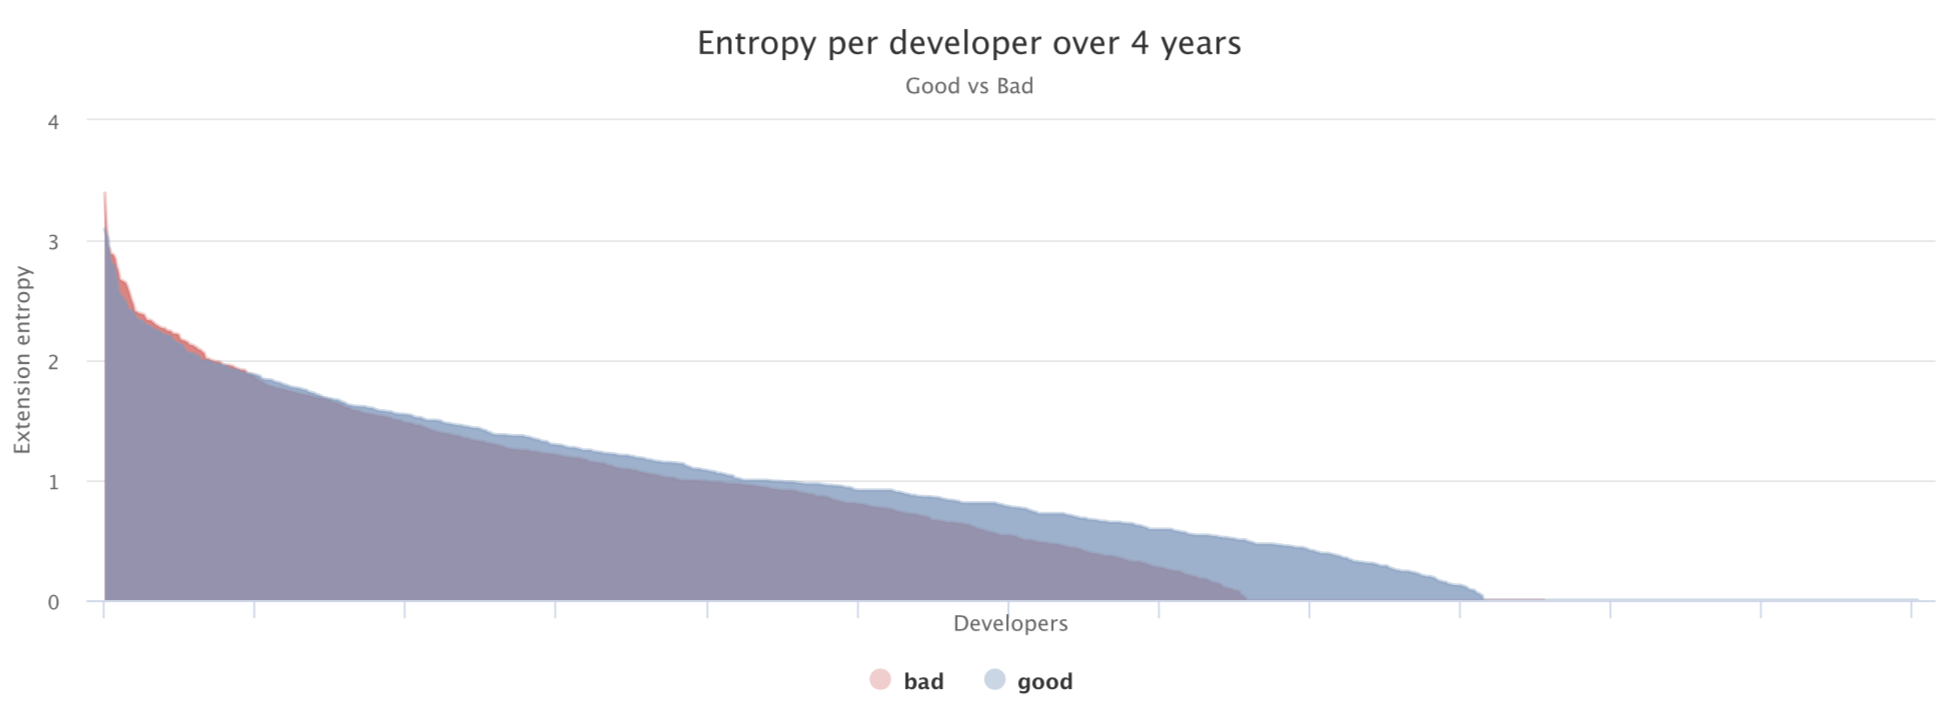
\includegraphics[width=1\textwidth]{figures/overall}
  \caption[Focus over 4 years]{The chart depicts the entropy levels for developers over 4 years (2014 - 2017). Over such a long time period, the difference in focus between two groups of developers disappears. This indicates that even though \textit{good developers} tend to focus on a specific technology over shorter periods of time, they do not monopolize their attention overall.} \label{fig:overall}
\end{figure}

\textit{Good developers} tended to focus on one task, finish it, and then move on to the next one. They did not stick to working exclusively on one technology over four years, but they focused during limited periods of time, namely daily or yearly. In this paper, the assumption is made that if developers diversified the extensions over four years, they diversified them over longer amount of time as well. This is why the claim is made that \textit{good developers} did not monopolize their attention to small set of technologies over their careers. The difference in focus of \textit{good} and \textit{bad developers} was clearly visible on a daily basis, less but still visible on the yearly basis, as depicted in \autoref{fig:daily} and \autoref{fig:yearly_2014}.

\begin{figure}[htpb]
  \centering
  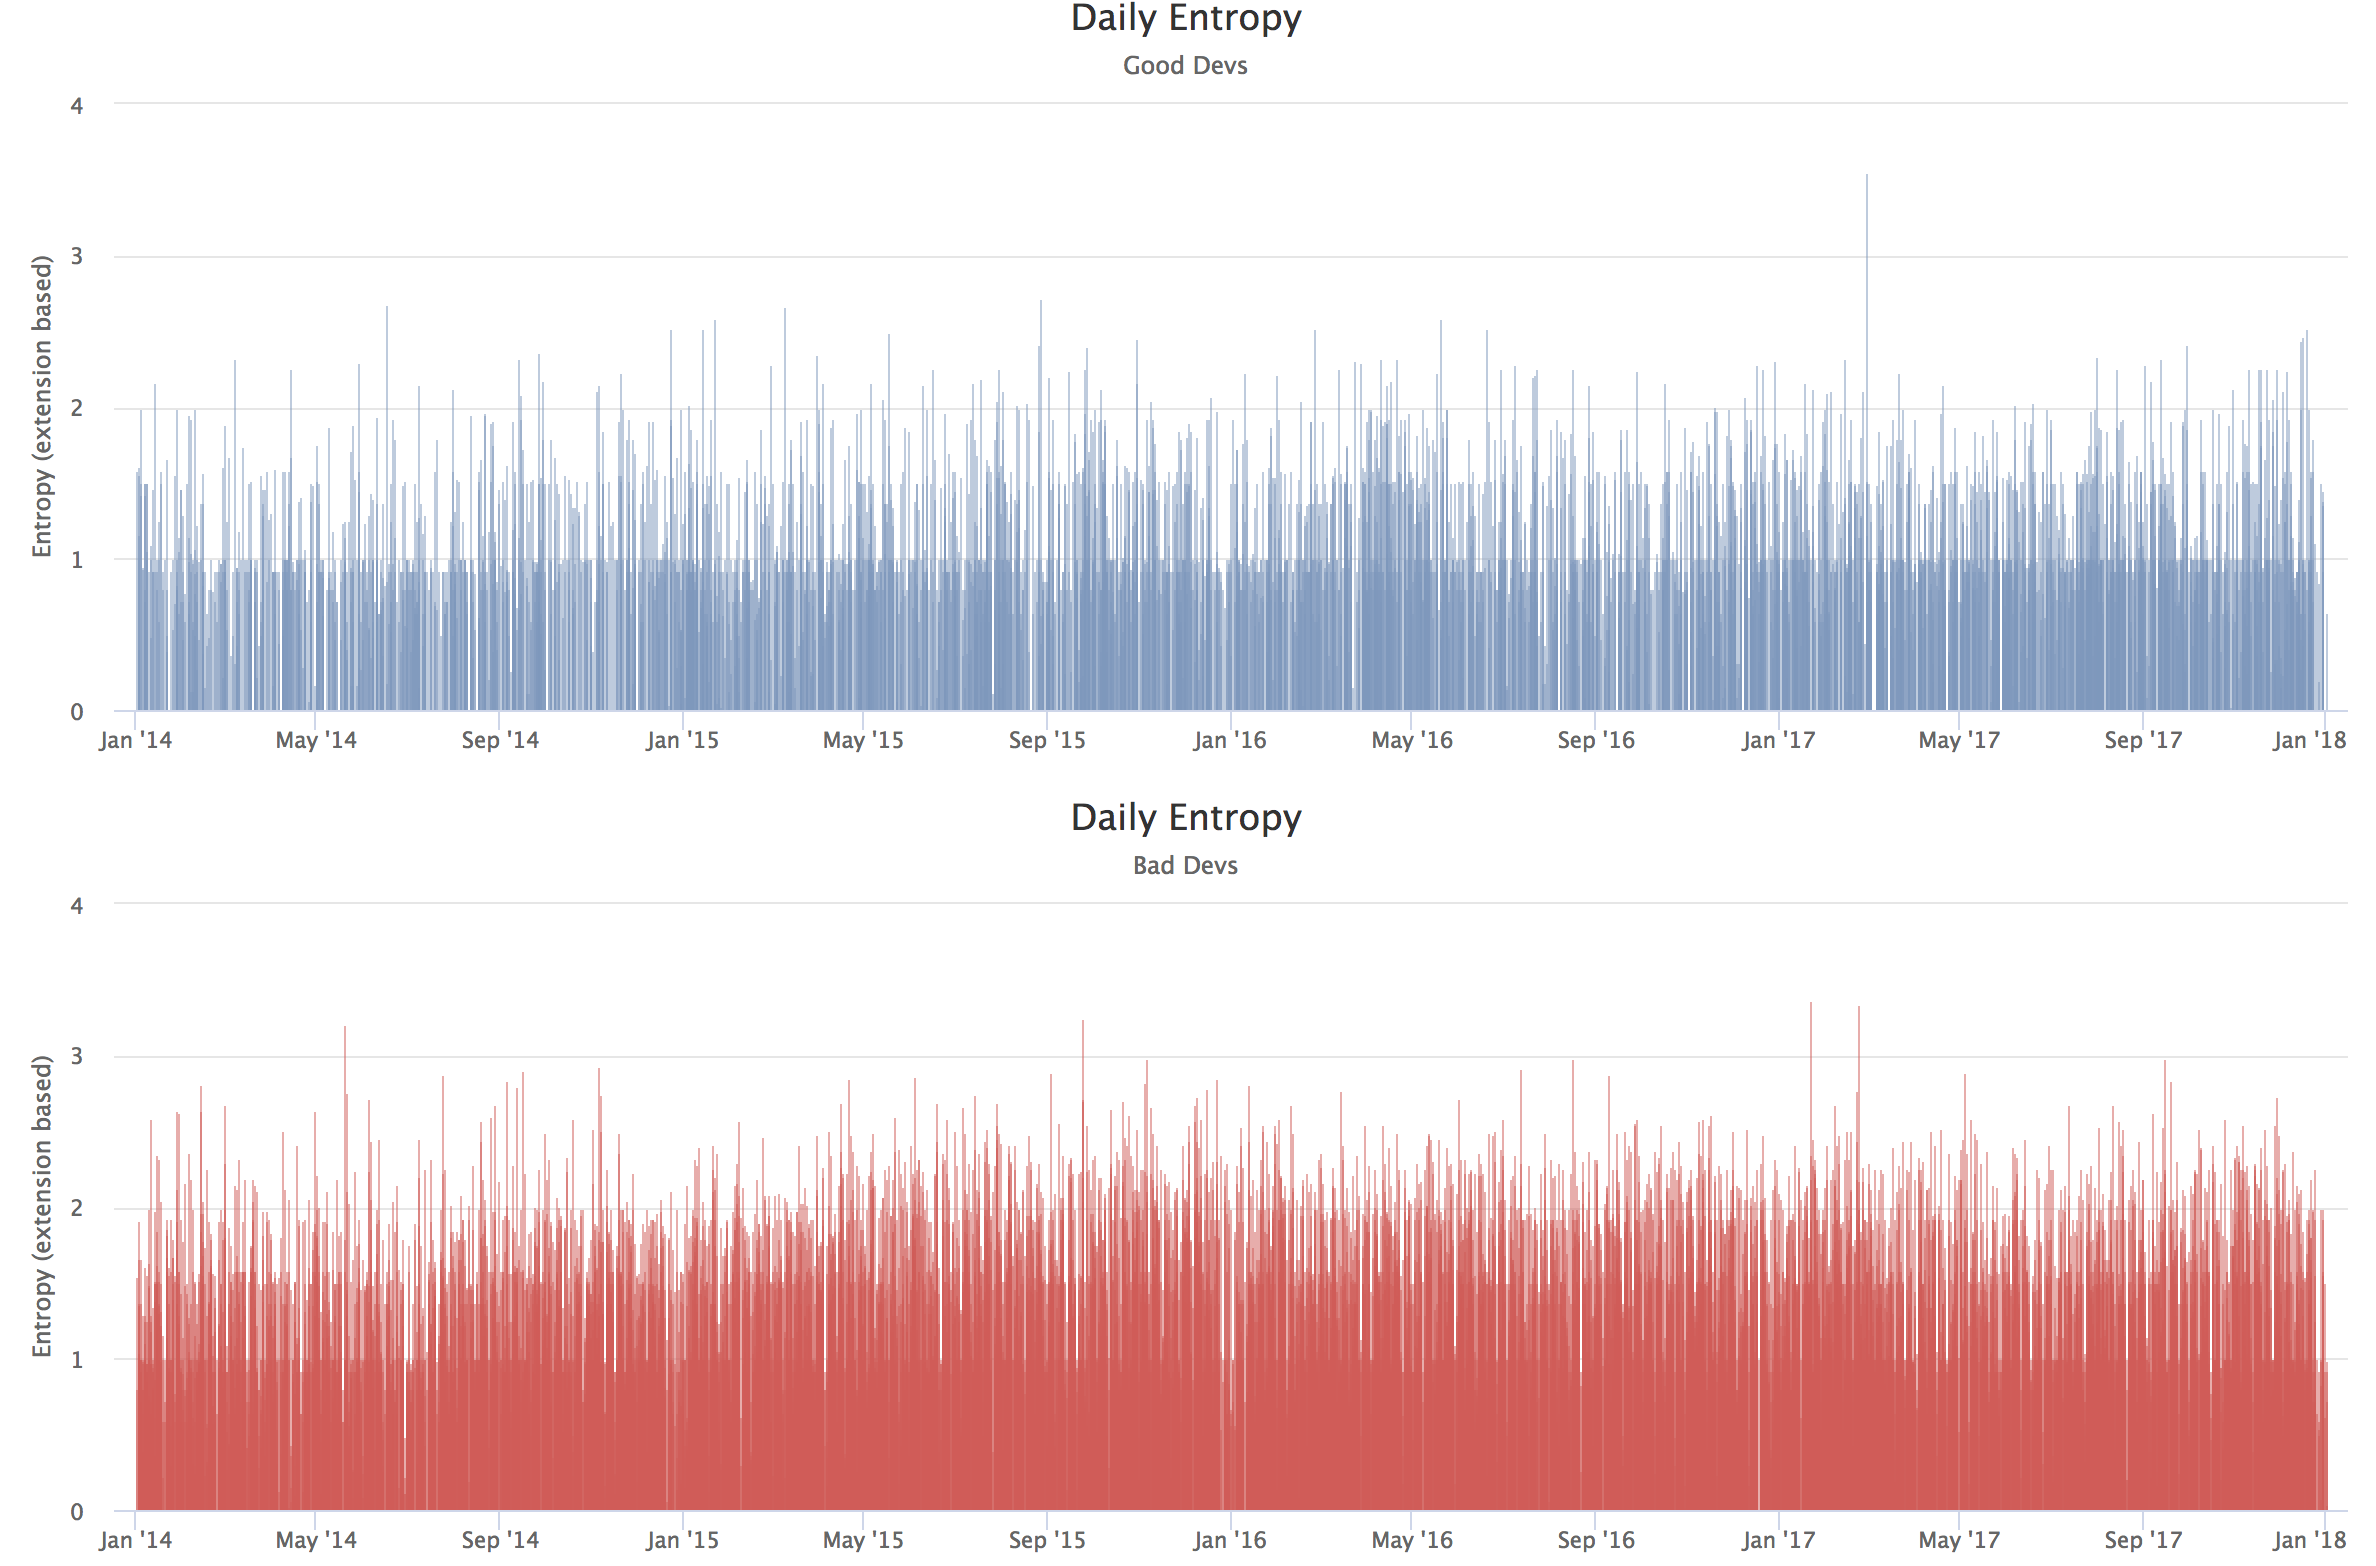
\includegraphics[width=1\textwidth]{figures/daily}
  \caption[Daily Focus Chart]{The two charts display daily entropy values for \textit{good} and \textit{bad developers}. The y-axis represents entropy and x-axis represents the developer-date combination. Each vertical line displays en entropy value for a developer for a specific day. It is clearly visible that \textit{good developers} are more focused on the daily basis. The area between entropy level 1 and 2 is mostly filled for \textit{bad developers}, while it is just partially covered for \textit{good developers}, since not many \textit{good developers} reach such a high entropy value. Additionally, much larger percentage of bad developers has entropy beyond 2. Because lower entropy indicates higher focus, it can be deduced from the chart that \textit{good developers} display higher level of daily focus.} \label{fig:daily}
\end{figure}

\begin{figure}[htpb]
  \centering
  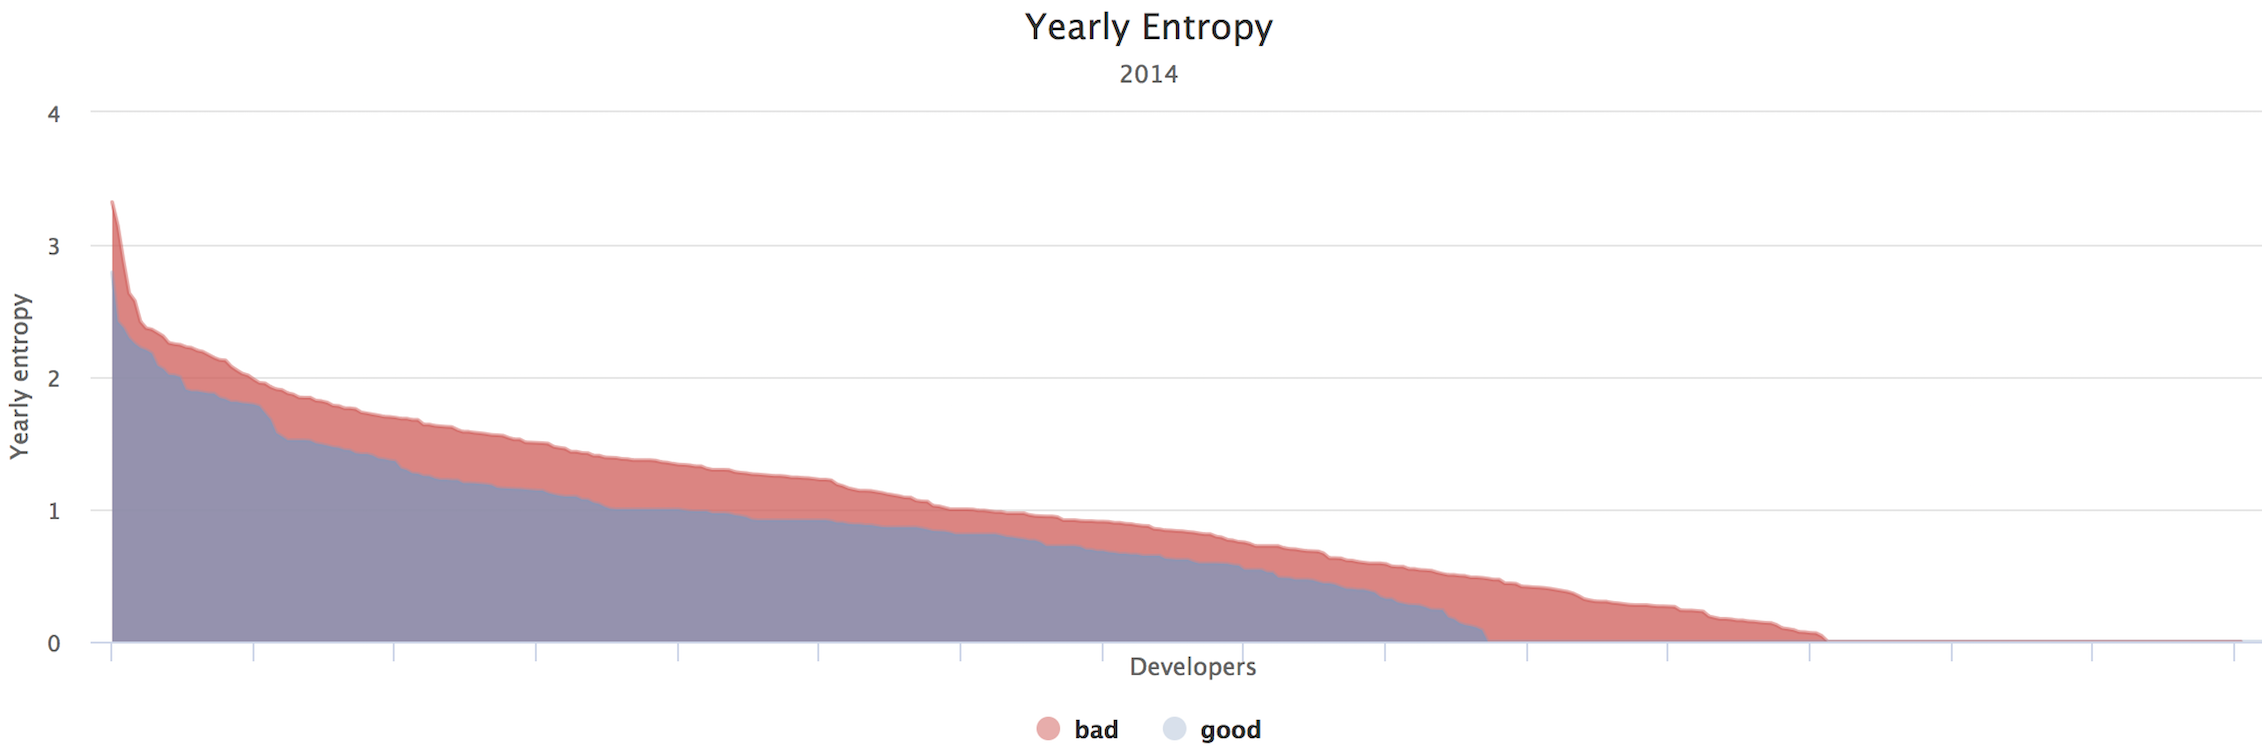
\includegraphics[width=1\textwidth]{figures/yearly_2014}
  \caption[Yearly Focus Chart for 2014]{Yearly entropy values for \textit{good} and \textit{bad developers} displayed as overlapping area charts for year 2014. Even on the yearly basis the good developers are more focused, although the difference is much less visible than with daily analysis. The charts for all four years can be found in the appendix.} \label{fig:yearly_2014}
\end{figure}

\subsection{RQ2: Are developers’ daily tasks within the week dependent on each other?}

A majority of developers from both groups scheduled daily tasks in a dependent way during the week. This means that their Friday work was dictated by their focus over the previous days in a week. This part of the research returned similar results for authors from both groups. According to the analysis, for 71\% of 2104 good developers, their focus on one day was dictated by work done on the previous days. Only 29\% of developers had independent days. Similarly, 66\% of 956 bad developers had dependent days, and for 33\% of them each day was independent. \par

On average, a \textit{good developer} worked on 3.31 different extensions over the four-year period, while a \textit{bad developer} worked on 6.41– almost twice as many. The next section describes the results of focus analysis per extension. \par

%%%%%%%%%%%%%%%%%%%%%%%%%%%%%%%%%%%%%%%%%%%%%%%%%%%%%%%%%%%%%%%%%%%%%%%%
\section{Focus per Extension}

Generally, entropy numbers per extension for \textit{bad developers} were much higher than for the other group, which indicated lower focus of \textit{bad developers}, as can be seen on  \autoref{fig:extensions}. 

\begin{figure}[htpb]
  \centering
  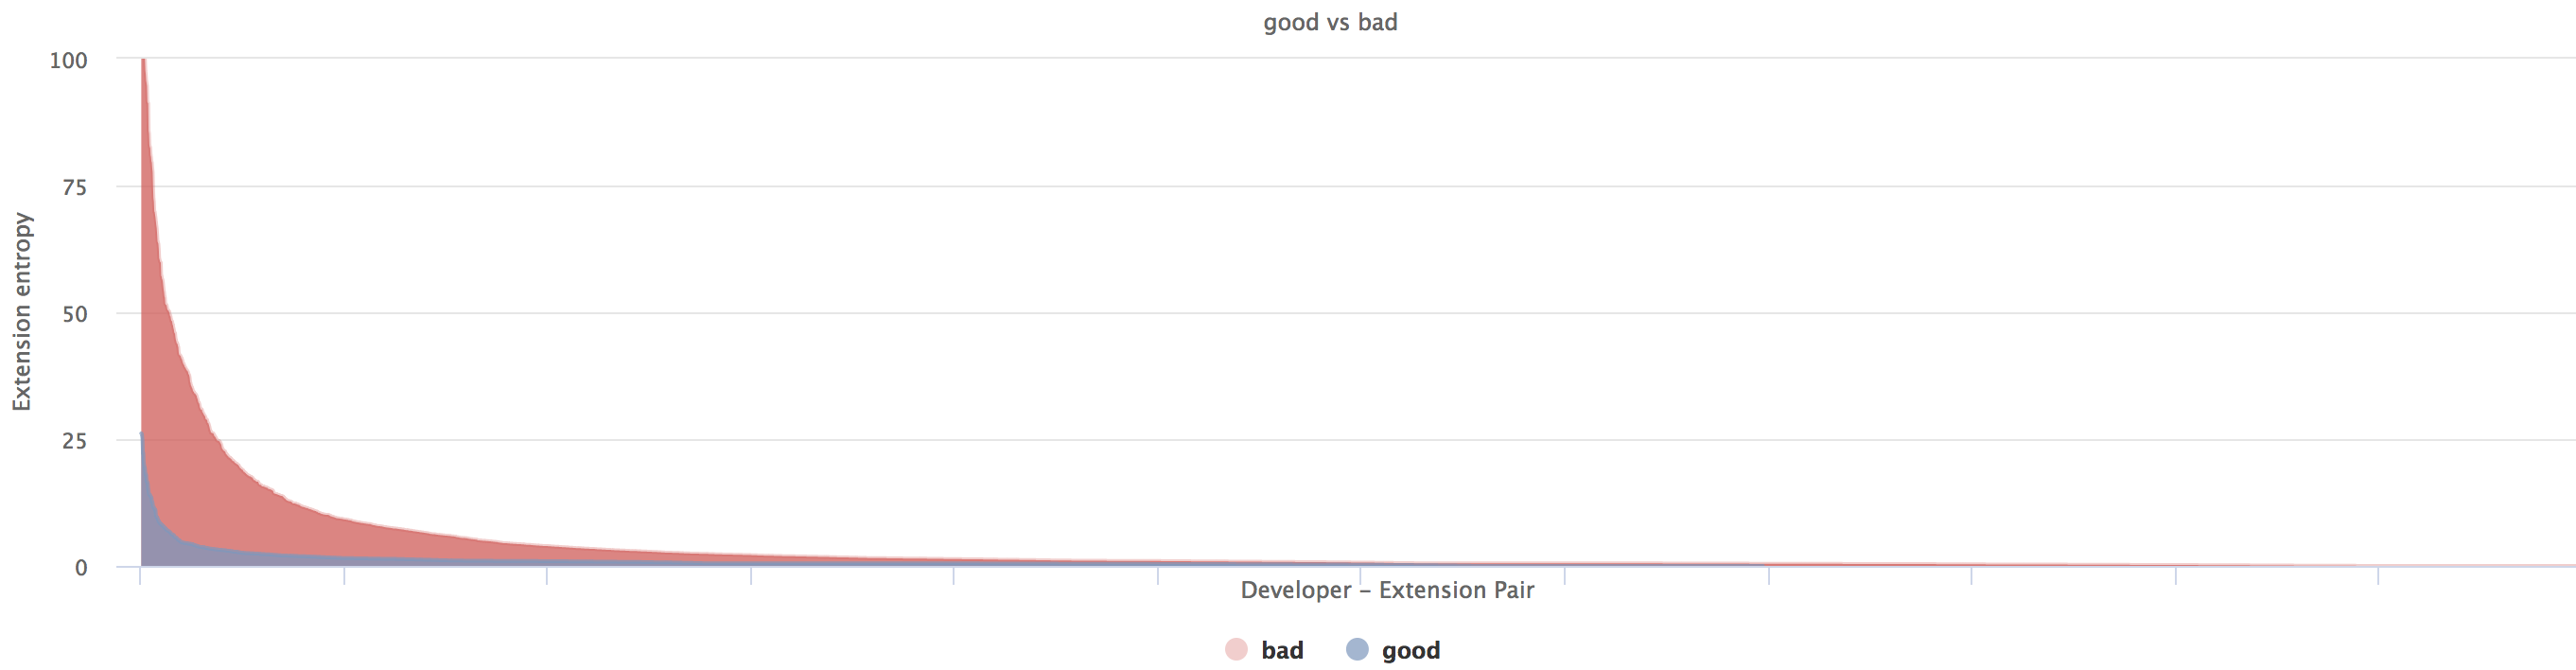
\includegraphics[width=1\textwidth]{figures/extensions}
  \caption[Focus Per Extension]{The graph depicts entropy values for the developer-extension pairs. The x-axis contains the developer-extension pair, while y-axis has the entropy value for the pair. The entropy for \textit{bad developers} went up to 188 for a few extreme cases, while the maximum for \textit{good developers} was 25. General higher numbers for \textit{bad developers} suggest that they do not focus on one specific extension, but work on multiple daily. To recall, the highest entropy numbers mean that developer was distributing the focus evenly across the extensions. These results are consistent with the previous analysis. } \label{fig:extensions}
\end{figure}

Entropy values for \textit{bad developers} went up to 188 on the extreme end. Comparatively, a few entropy scores for \textit{good developers} went up to 26 on the extreme end. To recall, this part of the analysis fixed developer-extension pair to discover developer’s focus per extension. \autoref{fig:extensions_zoom} displays a zoomed-in version of the previous chart to show clearly the difference in values for lower entropy (the long slim part of the graph along the x-axis).

\begin{figure}[htpb]
  \centering
  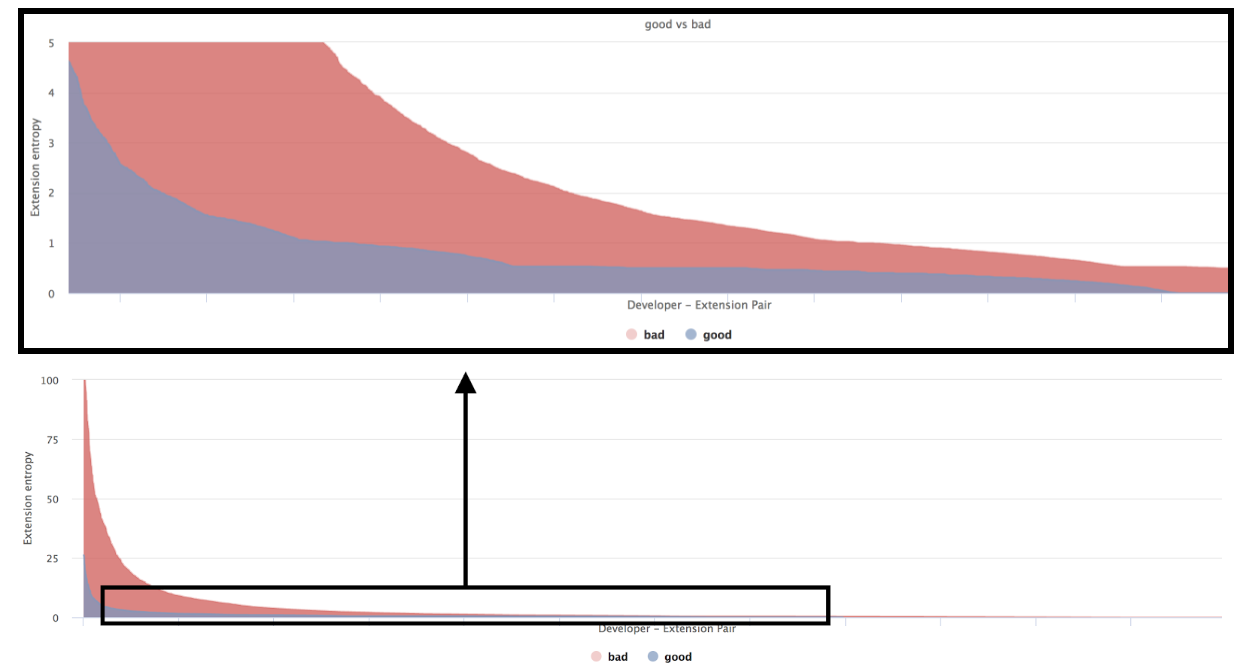
\includegraphics[width=1\textwidth]{figures/ext_zoom}
  \caption[Focus Per Extension For Lower Entropy Values]{The chart displays a portion of the entropy per extension chart from \autoref{fig:extensions} to emphasize the difference between low entropy values of \textit{good} and\textit{ bad developers}. The graph clearly shows that entropy values for \textit{bad developers} were higher. For \textit{good developers}, 78.27\% of developer-extension pairs have an entropy value below 1. To compare, for \textit{bad developers}, only 8.54\% have entropy value below 1.} \label{fig:extensions_zoom}
\end{figure}

Entropy values for the majority of \textit{bad developers} were between 0 and 5, with only 8.54\% being at or below 1. For \textit{bad developers}, 86.37\% of developer-extension pairs were at or below entropy value of 5, and 92.44\% were at or below entropy value of 10. Comparatively, a majority of \textit{good developers}’ entropy numbers were at or below 1. For \textit{good developers}, 78.27\% of developer-extension pairs were at or below entropy value of 1, and 90.82\% were at or below entropy value of 2. Entropy ranges and the respective numbers of developer-extension pairs for each group are displayed in \autoref{table:extensions} . 

\begin{table}[h!]
\begin{center}
\begin{tabular}{ |p{5cm}|p{4cm}|p{4cm}|  }
 \hline
 Entropy Range &
 \multicolumn{2}{c|}{Number of Developer-Extension Pairs} \\
 & \textit{Good Developers} & \textit{Bad Developers}\\
 \hline \hline
 0   & 690    & 523 \\
 0 < entropy <= 1 &   2430  & 3229 \\
 1 < entropy <= 2 & 500 & 834\\
 2 < entropy <= 5  & 271 & 706\\
 5 < entropy <= 10 &   59 & 372  \\
 10 < entropy <= 20 & 29  & 226  \\
 20 < entropy <= 50 & 7  & 167 \\
 50 < entropy <= 100 &   0 & 61  \\
 100 < entropy <= 200 &   0 & 9  \\
 \hline
\end{tabular}
\end{center}
\caption[Entropy Ranges. Focus Per Extension]{The table displays ranges of entropy values and corresponding number of developer-extension pairs for \textit{good} and \textit{bad developers}. Clearly, majority of pairs for \textit{good developers} is between 0 and 1. To compare, majority of pairs is between 0 and 5 for \textit{bad developers}.}
\label{table:extensions}
\end{table}

\subsection{RQ3: Are good developers more focused when working on the most popular extensions?}

Among the 10 most popular extensions, \textit{good developers} focused on all of them more than \textit{bad developers}. In general, there was a large difference in focus for all popular extensions except .rb. The focus for both groups was similar for the Ruby extension–even \textit{good developers} displayed lower focus. The most popular extensions for the developers in the data set included .java, .js, .json, .lock, .md, .py, .rb, .rs, .txt, and .yml. Some of the extensions are utilized for documentation rather than coding like .txt or .md. Json format may be argued to be a data file that should not be used in the analysis, however, a lot of Javascript and TypeScript frameworks use it for configuration and that is why the extension was included in this part of the research. The .lock extension is used by the operating systems to limit concurrent access to resources so it is excluded from discussion. Otherwise, the popular extensions are not surprising considering that those are the extensions of the majority of the languages from the selected repositories, plus documentation and configuration. The popular extensions were chosen from the pool of all the authors, so some of the extensions were used more by one group and some by the other. \autoref{fig:java_log} presents developers' focus chart for .java extension. For comparison, \autoref{fig:rb_log} shows the chart for .rb. There were less \textit{good developers} working on all of the popular extensions except for .rb, .md and .rs. The charts for all the extensions can be seen in the Appendices. \par

\begin{figure}[htpb]
  \centering
  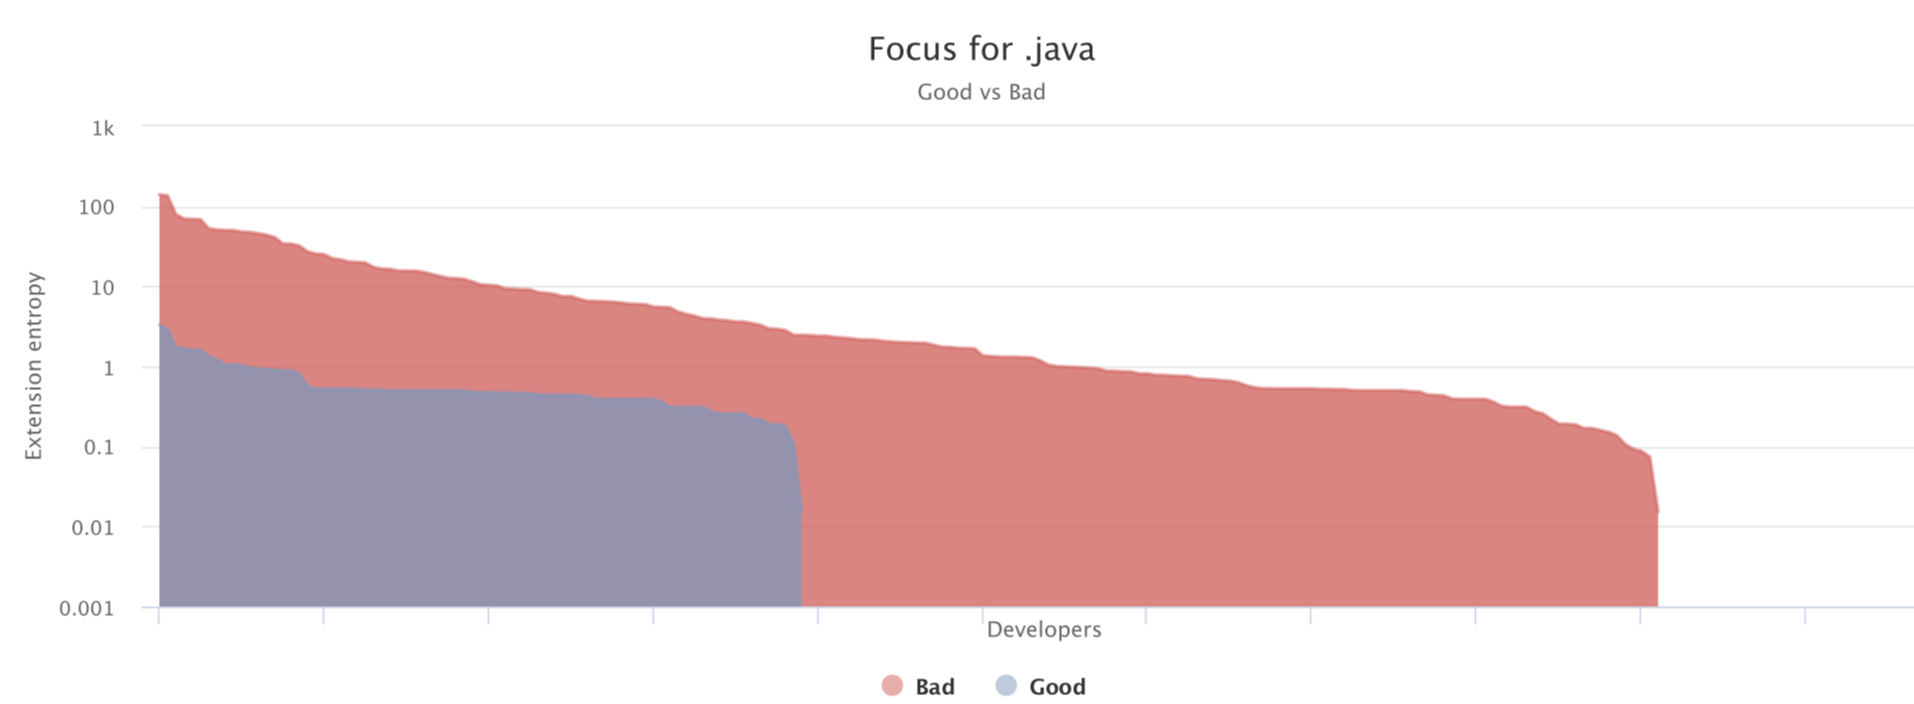
\includegraphics[width=1\textwidth]{figures/java_log}
  \caption[Focus for .java]{The graph depicts .java entropy levels for developers from both groups using logarithmic y-axis. Clearly, \textit{good developers} are more focused on the Java files.  It is easy to perceive that more \textit{bad developers} work on .java extensions than good developers.} \label{fig:java_log}
\end{figure}

\begin{figure}[htpb]
  \centering
  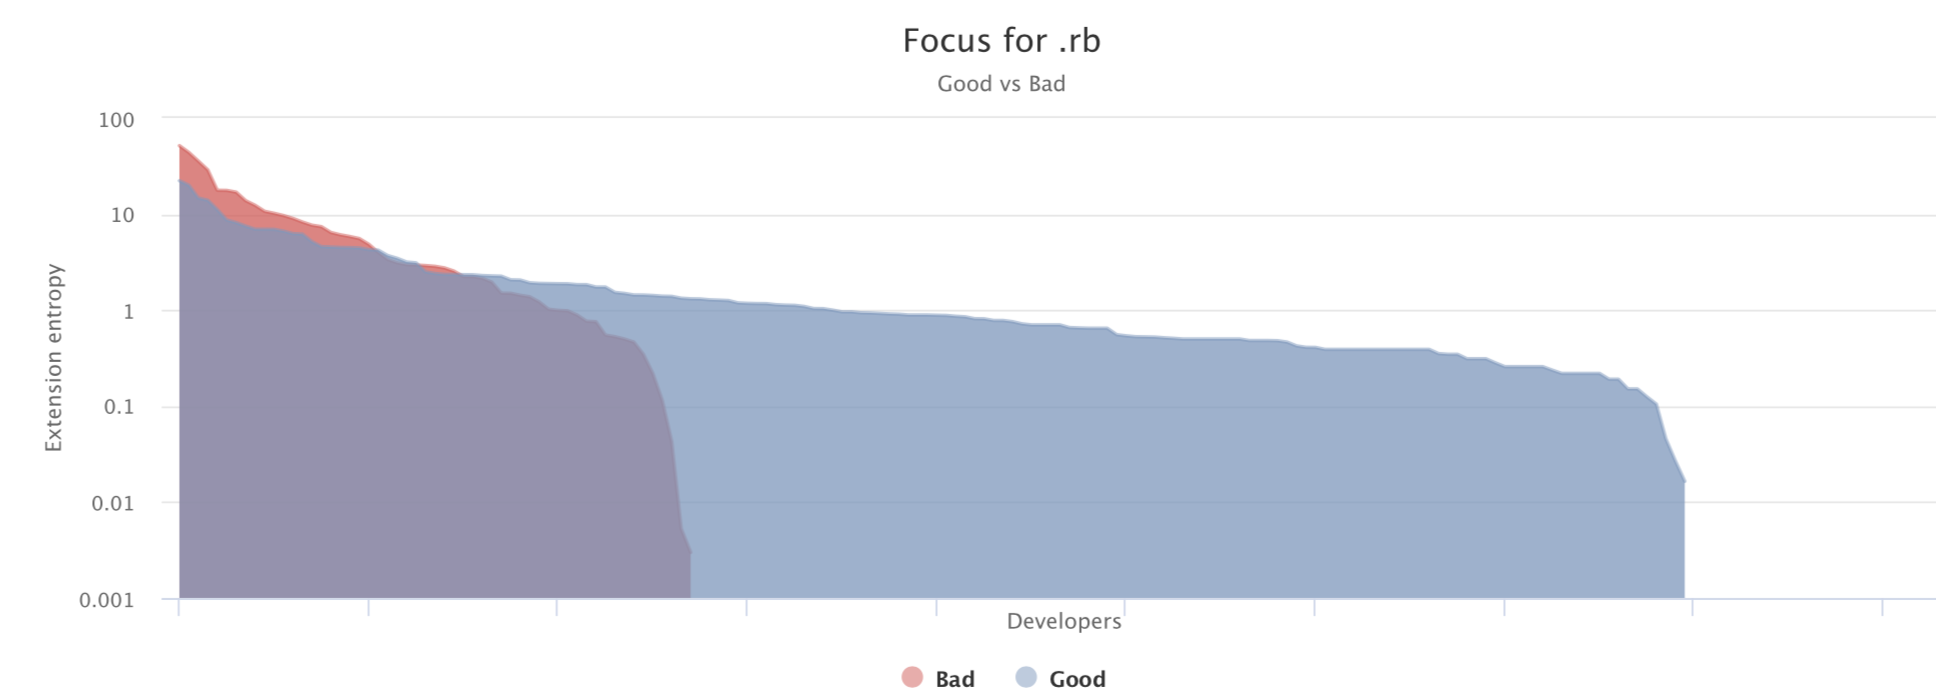
\includegraphics[width=1\textwidth]{figures/rb_log}
  \caption[Focus for .rb]{The graph depicts .rb entropy levels for developers from both groups using logarithmic y-axis. The level of focus on Ruby files is very similar for \textit{good} and \textit{bad developers}. Evidently, more \textit{good developers} work on the .rb extension.} \label{fig:rb_log}
\end{figure}

\subsection{RQ4: Which extensions do good developers focus on the most?}

\textit{Good developers} focus the most on the following file extensions: .bat, .map, .rc, .sql, .policy.   The list contains a combination of configuration files, batch scripts and database scripts. The extensions relate to variety of technologies including command line scripting, SQL, Visual Studio, C++, Java, Html, Sass and game interfaces. For each of these extensions, entropy was checked for the opposite group and it was discovered that \textit{bad developers} were less focused on all of them. \par

To recall, the extensions with average entropy of below 0.3 are considered as those the developers focus on the most. Additionally, binary extensions were excluded from the result list. \par

It was hard to find the extensions which \textit{ bad developers} focus on the most because entropy values were generally much higher than in case of \textit{good developers}. There was no extension that \textit{bad developers }were the most focused on when applying the original criteria. The results are displayed in \autoref{table:focused}. 

\begin{table}[h!]
\begin{center}
\begin{tabular}{ | m{5em} | m{15em}| m{15em}| } 
\hline
Group & Most focused (entropy < 0.3) & Corresponding extensions entropy from other group \\ 
\hline \hline
\multirow{5}{4em}{\textit{Good}} & .map 0.261940, &  \\
& .bat 0.239284  &  \\
& .rc 0.278828 &  \\
& .sql 0.283274&  \\
& .policy 0.245950  &  \\
\hline
\multirow{5}{4em}{\textit{Bad}} &  & .map 1.797670 \\ 
&  & .bat 0.913662  \\
& & .rc 1.626362  \\
&  &  .sql 0.842708\\
&   &  .policy 1.691119 \\
\hline
\end{tabular}
\end{center}
\caption[Extensions that Developers Focus on the Most]{The extensions that developers focus on the most (entropy < 0.3). Average entropy across developers in the group was used as a measure. The third column displays the entropy results for the extensions from the other group for comparison. Using 0.3 as the entropy threshold, no extensions were found for \textit{bad developers}.}
\label{table:focused}
\end{table}

To further investigate the extensions which \textit{bad developers} focus on the most, additional analysis was done with higher entropy level. Using 0.6 as the entropy threshold, \textit{bad developers} focus the most on the following extensions: .po, a properties file used in Java, and .coffee, a CoffeeScript file that compiles into Javascript.  Once the entropy threshold is raised so high, there are numerous extensions that \textit{good developers} focus on. \autoref{table:focused_extended} contains the list of additional file extensions developers focus on the most using the new, higher entropy threshold. That list does not include the extensions enumerated in the previous table. For \textit{good developers}, the extensions are a mix of configuration and build related files and some major file extensions from known programming languages like C, C++, TypeScript, C\# or Java. 

\begin{table}[htpb]
\begin{center}
\begin{tabular}{ | m{20em} | m{20em}| } 
\hline
\textit{Good Developers} & \textit{Bad Developers} \\ 
\hline \hline
.conf 0.3197320635055236 & .po 0.5514069703162789\\
.cc 0.33219280948873625 & .coffee 0.48716161553142023 \\
.tsx 0.32548038205462104 & \\
.cs 0.335181806848358  & \\
.po 0.3771562013985646 & \\
.rst 0.38434150516100074 & \\
.java 0.38668939720297063  & \\
.cfg 0.4150984518773275  & \\
.css 0.4331270566825627 & \\
.csproj 0.45364909626365557 & \\
.properties 0.46818206642405324 & \\
.xsd 0.4694220594512273 & \\
.adoc 0.4811941129621413  & \\
.c 0.48835032030656583  & \\
.gradle 0.4981850663754806  & \\
.desc 0.5380845749665812  & \\
.ui 0.5605287497175695 & \\
.htm 0.5729759329981284 & \\
.rake 0.5894723449699876 & \\
\hline
\end{tabular}
\end{center}
\caption[Extended Extensions that Developers Focus on the Most]{Additional extensions that developers focus on the most excluding the ones from previous table ( 0.3 < entropy < 0.6). Average entropy across developers in the group was used as a measure. Clearly \textit{good developers} display significant focus for larger amount of extensions.}
\label{table:focused_extended}
\end{table}

Developers from two groups differed in their focus per extension. Out of all the extensions, they interacted with .csproj in the most different way, with \textit{good developers} being more focused on it. It should be noted that C\# project files can be modified directly by developers, but they can also be automatically changed by an IDE.






